\documentclass[conference]{IEEEtran}
\IEEEoverridecommandlockouts
\usepackage{cite}
\usepackage{amsmath,amssymb,amsfonts}
\usepackage{algorithmic}
\usepackage{graphicx}
\usepackage{textcomp}
\usepackage{xcolor}
\usepackage{url}
\usepackage{tikz}
\usepackage{pgfplots}
\pgfplotsset{compat=1.18}

% TikZ libraries
\usetikzlibrary{shapes.geometric, arrows.meta, positioning, calc, shapes.symbols}

% Define colors
\definecolor{primaryblue}{RGB}{0,102,204}
\definecolor{secondarygreen}{RGB}{76,175,80}
\definecolor{accentorange}{RGB}{255,152,0}

% Define TikZ styles
\tikzstyle{process} = [rectangle, rounded corners, minimum width=2.5cm, minimum height=1cm, text centered, draw=black, fill=blue!20, font=\small]
\tikzstyle{decision} = [diamond, minimum width=2cm, minimum height=1cm, text centered, draw=black, fill=green!20, font=\small]
\tikzstyle{data} = [trapezium, trapezium left angle=70, trapezium right angle=110, minimum width=2cm, minimum height=0.8cm, text centered, draw=black, fill=gray!20, font=\small]
\tikzstyle{database} = [cylinder, shape border rotate=90, aspect=0.25, minimum width=2cm, minimum height=1.2cm, text centered, draw=black, fill=green!20, font=\small]
\tikzstyle{arrow} = [thick,->,>=stealth]

\def\BibTeX{{\rm B\kern-.05em{\sc i\kern-.025em b}\kern-.08em
    T\kern-.1667em\lower.7ex\hbox{E}\kern-.125emX}}
\begin{document}

\title{TalentBridge: An AI-Powered Intelligent Job Matching Platform for Vietnamese Students Using Semantic Search and Large Language Models}

\author{\IEEEauthorblockN{Trinh Van Hao, Phan Xuan Khai}
\IEEEauthorblockA{\textit{Faculty of Information Technology} \\
\textit{Dai Nam University}\\
Hanoi, Vietnam \\
haotrinh142@gmail.com}
}

\maketitle

\begin{abstract}
The job search process for students often faces challenges due to information asymmetry and inefficient matching between candidate skills and job requirements. This paper presents TalentBridge, an intelligent job matching platform that leverages Google Gemini AI and semantic search technologies to automate CV analysis, provide personalized job recommendations, and deliver actionable career insights. The system employs a hybrid approach combining Large Language Models (LLMs) for CV parsing and quality assessment with vector embeddings for semantic job matching. Experimental results on a dataset of 3,237 real job postings demonstrate that our approach achieves high accuracy in CV information extraction and provides meaningful job recommendations with explainable AI-generated matching scores. The platform features automatic CV parsing from PDF documents, multi-dimensional quality scoring, semantic-based job matching, and comprehensive market analytics, all optimized for Vietnamese students and the Vietnamese job market.
\end{abstract}

\begin{IEEEkeywords}
job matching, semantic search, large language models, CV analysis, recommendation systems, vector embeddings, career analytics
\end{IEEEkeywords}

\section{Introduction}

The transition from university to the workforce represents a critical challenge for students worldwide. In Vietnam, students face particular difficulties in identifying suitable job opportunities that match their skills, experience, and career aspirations. Traditional job search platforms rely primarily on keyword-based search, which often fails to capture the semantic relationships between candidate qualifications and job requirements \cite{b1}.

Recent advances in Large Language Models (LLMs) and vector embeddings have opened new possibilities for intelligent job matching systems. These technologies enable deeper understanding of both CV content and job descriptions, facilitating more accurate matching beyond simple keyword overlap \cite{b2}.

This paper presents TalentBridge, an AI-powered platform specifically designed for Vietnamese students that addresses three key challenges. First, manual CV review is time-consuming and subjective, so our system uses Google Gemini 2.5 Flash to automatically extract structured information from PDF documents, enabling CV analysis automation. Second, traditional keyword search fails to capture semantic similarity, which is why we employ 768-dimensional vector embeddings with ChromaDB for semantic job matching. Third, black-box recommendation systems lack transparency, so our platform provides AI-generated explanations for each job match to ensure explainable recommendations.

The main contributions of this work include a novel hybrid architecture combining LLMs for CV parsing with vector embeddings for semantic matching, a multi-dimensional CV quality assessment framework with three scoring metrics, an explainable job recommendation system with AI-generated matching rationales, a comprehensive analytics dashboard providing market insights for students, and implementation and evaluation on real Vietnamese job market data covering 3,237 positions.

\section{Related Work}

\subsection{Job Recommendation Systems}

Traditional job recommendation systems employ collaborative filtering \cite{b3} or content-based filtering approaches. Recent work has explored deep learning methods including neural collaborative filtering and graph neural networks \cite{b4}. However, these approaches often require extensive user interaction history and struggle with cold-start problems for new graduates.

\subsection{CV Parsing and Information Extraction}

CV parsing has been addressed using rule-based systems, Named Entity Recognition (NER), and more recently, transformer-based models \cite{b5}. Commercial solutions like Sovren and Textkernel provide CV parsing APIs, but they are expensive and not optimized for Vietnamese CVs.

\subsection{Semantic Search with Vector Embeddings}

Vector embeddings have revolutionized semantic search across various domains \cite{b6}. Recent embedding models like Google's text-embedding-004 achieve state-of-the-art performance on semantic similarity tasks. ChromaDB and similar vector databases enable efficient similarity search at scale.

\section{System Architecture}

\subsection{Overview}

TalentBridge employs a three-tier architecture consisting of: (1) Frontend layer with HTML/JavaScript interface, (2) Backend API layer built with FastAPI, and (3) Data layer combining SQLite for structured data and ChromaDB for vector storage. Figure~\ref{fig:architecture} illustrates the complete system architecture with all major components and their interactions.

\subsection{Backend Components}

\subsubsection{API Layer}
The FastAPI backend exposes over 15 RESTful endpoints for CV upload, job search, matching, and analytics. Key endpoints include \texttt{POST /upload-cv} for CV upload and parsing, \texttt{POST /match} for semantic job matching, and \texttt{GET /jobs/analytics} for market analytics.

\subsubsection{AI Analysis Module}
This module integrates Google Gemini AI with three primary functions. The CV parsing function extracts structured information including personal details, skills, education, and experience from PDF documents. The quality assessment function generates three scores covering quality, market fit, and completeness with detailed feedback. The job ranking function scores job-candidate matches on a 0-1 scale with explanations.

\subsubsection{Vector Search Module}
ChromaDB stores 768-dimensional embeddings for all job postings. The semantic matching pipeline operates in four stages: first, it generates CV embedding using text-embedding-004; second, it queries ChromaDB for top-k similar jobs using cosine similarity; third, it re-ranks results using Gemini AI; and finally, it generates explanations for top matches.

\subsection{Database Schema}

The SQLite database contains six tables: \texttt{cv\_store} for parsed CV data in JSON format, \texttt{job\_store} for job postings containing 3,237 records, \texttt{cv\_insights} for quality scores and feedback, \texttt{match\_logs} for matching history, \texttt{applications} for application tracking, and \texttt{analytics\_cache} for cached statistics.

\subsection{Frontend Interface}

The frontend consists of four main pages. The landing page provides job search and category browsing functionality. The CV analysis page handles upload, parsing, and quality assessment. The job listing page enables users to search, filter, and browse positions. The dashboard page displays market analytics with six chart types.

% FIGURE 1: System Architecture
\begin{figure*}[t]
\centering
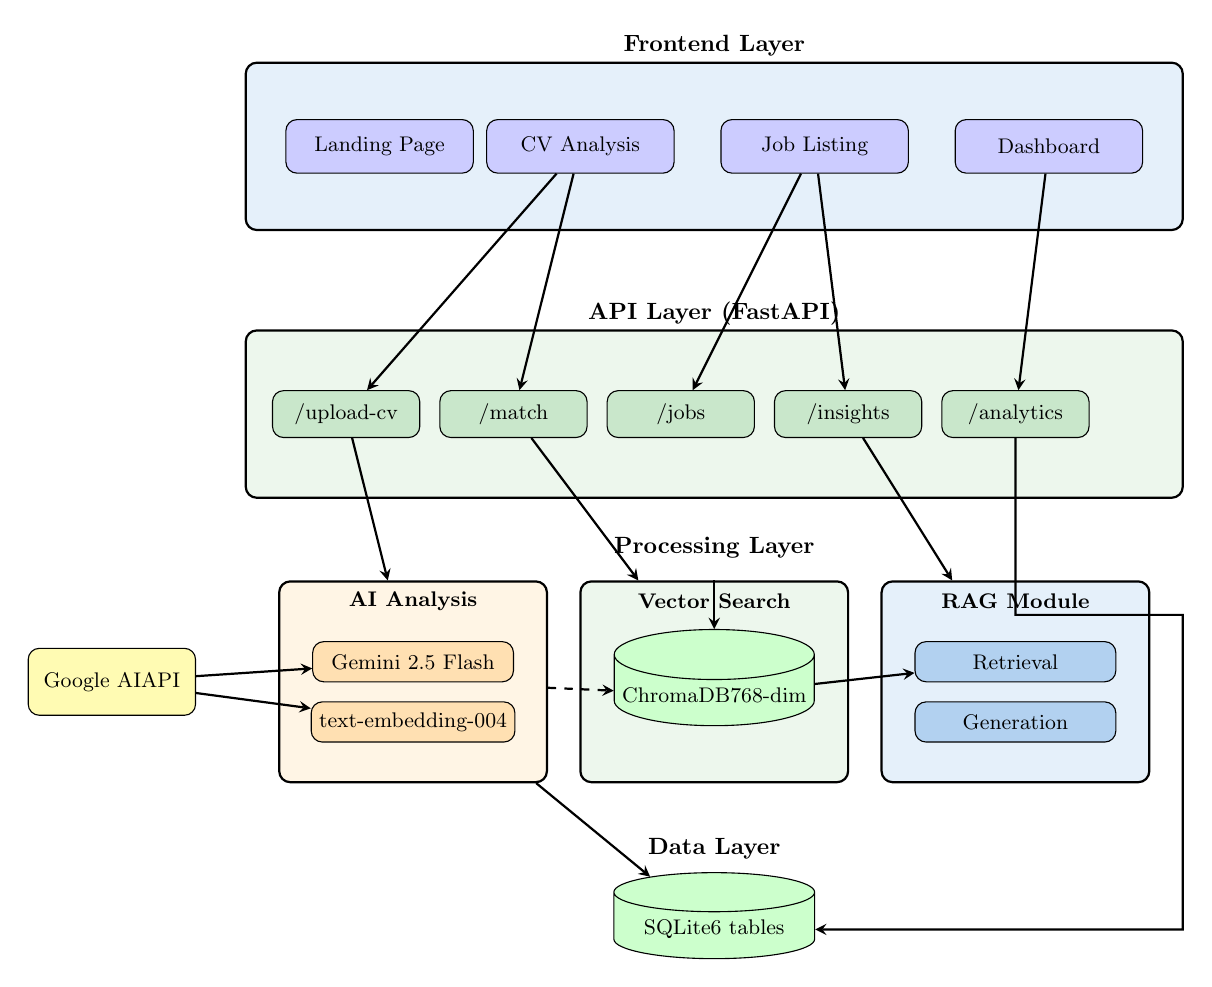
\begin{tikzpicture}[node distance=2cm, scale=0.85, every node/.style={scale=0.85}]

% ===== FRONTEND LAYER =====
\node (frontend_label) [draw=none, fill=none, font=\bfseries] at (0, 0) {Frontend Layer};
\node (frontend_box) [draw, thick, rounded corners, minimum width=14cm, minimum height=2.5cm, fill=primaryblue!10] at (0, -1.5) {};

\node (index) [process, minimum width=2.8cm, minimum height=0.8cm] at (-5, -1.5) {Landing Page};
\node (cvpage) [process, minimum width=2.8cm, minimum height=0.8cm] at (-2, -1.5) {CV Analysis};
\node (jobpage) [process, minimum width=2.8cm, minimum height=0.8cm] at (1.5, -1.5) {Job Listing};
\node (dashboard) [process, minimum width=2.8cm, minimum height=0.8cm] at (5, -1.5) {Dashboard};

% ===== API LAYER =====
\node (api_label) [draw=none, fill=none, font=\bfseries] at (0, -4) {API Layer (FastAPI)};
\node (api_box) [draw, thick, rounded corners, minimum width=14cm, minimum height=2.5cm, fill=secondarygreen!10] at (0, -5.5) {};

\node (upload) [process, minimum width=2.2cm, minimum height=0.7cm, fill=secondarygreen!30] at (-5.5, -5.5) {/upload-cv};
\node (match) [process, minimum width=2.2cm, minimum height=0.7cm, fill=secondarygreen!30] at (-3, -5.5) {/match};
\node (jobs) [process, minimum width=2.2cm, minimum height=0.7cm, fill=secondarygreen!30] at (-0.5, -5.5) {/jobs};
\node (insights) [process, minimum width=2.2cm, minimum height=0.7cm, fill=secondarygreen!30] at (2, -5.5) {/insights};
\node (analytics) [process, minimum width=2.2cm, minimum height=0.7cm, fill=secondarygreen!30] at (4.5, -5.5) {/analytics};

% ===== PROCESSING LAYER =====
\node (processing_label) [draw=none, fill=none, font=\bfseries] at (0, -7.5) {Processing Layer};

% AI Module
\node (ai_box) [draw, thick, rounded corners, minimum width=4cm, minimum height=3cm, fill=accentorange!10] at (-4.5, -9.5) {};
\node (ai_label) [draw=none, fill=none, font=\small\bfseries] at (-4.5, -8.3) {AI Analysis};
\node (gemini) [process, minimum width=3cm, minimum height=0.6cm, fill=accentorange!30, font=\small] at (-4.5, -9.2) {Gemini 2.5 Flash};
\node (embedding) [process, minimum width=3cm, minimum height=0.6cm, fill=accentorange!30, font=\small] at (-4.5, -10.1) {text-embedding-004};

% Vector Module
\node (vector_box) [draw, thick, rounded corners, minimum width=4cm, minimum height=3cm, fill=secondarygreen!10] at (0, -9.5) {};
\node (vector_label) [draw=none, fill=none, font=\small\bfseries] at (0, -8.3) {Vector Search};
\node (chromadb) [database, minimum width=2.5cm, minimum height=1cm, font=\small] at (0, -9.7) {ChromaDB\\768-dim};

% RAG Module (NEW)
\node (rag_box) [draw, thick, rounded corners, minimum width=4cm, minimum height=3cm, fill=primaryblue!10] at (4.5, -9.5) {};
\node (rag_label) [draw=none, fill=none, font=\small\bfseries] at (4.5, -8.3) {RAG Module};
\node (rag_retrieval) [process, minimum width=3cm, minimum height=0.6cm, fill=primaryblue!30, font=\small] at (4.5, -9.2) {Retrieval};
\node (rag_generation) [process, minimum width=3cm, minimum height=0.6cm, fill=primaryblue!30, font=\small] at (4.5, -10.1) {Generation};

% ===== DATA LAYER =====
\node (data_label) [draw=none, fill=none, font=\bfseries] at (0, -12) {Data Layer};
\node (sqlite) [database, minimum width=3cm, minimum height=1.2cm] at (0, -13.2) {SQLite\\6 tables};

% External API
\node (google_api) [process, minimum width=2.5cm, minimum height=1cm, fill=yellow!30] at (-9, -9.5) {Google AI\\API};

% ===== ARROWS =====
% Frontend to API (logical connections)
\draw [arrow] (cvpage) -- (upload);
\draw [arrow] (cvpage) -- (match);
\draw [arrow] (jobpage) -- (jobs);
\draw [arrow] (jobpage) -- (insights);
\draw [arrow] (dashboard) -- (analytics);

% API to Processing (correct routing)
\draw [arrow] (upload) -- (ai_box);
\draw [arrow] (match) -- (vector_box);
\draw [arrow] (insights) -- (rag_box);

% Analytics goes around vector search box to avoid overlap
\draw [arrow] (analytics) -- ++(0,-3) -| ++(2.5,0) |- (sqlite);

% Processing to Data
\draw [arrow] (ai_box) -- (sqlite);
\draw [arrow] (vector_box) -- (chromadb);

% External API connections
\draw [arrow] (google_api) -- (gemini);
\draw [arrow] (google_api) -- (embedding);

% ChromaDB connections
\draw [arrow] (chromadb) -- (rag_retrieval);
\draw [arrow, dashed] (ai_box) -- (chromadb);

\end{tikzpicture}
\caption{TalentBridge System Architecture - Three-tier design with AI-powered backend and RAG module}
\label{fig:architecture}
\end{figure*}

\section{Methodology}

\subsection{CV Parsing with LLMs}

Traditional CV parsing relies on templates and regular expressions, which fail on diverse formats. We employ Gemini 2.5 Flash with structured prompts to extract CV data into JSON format. Figure~\ref{fig:cv_parsing_flow} shows the workflow.

The pipeline extracts: (1) personal information, (2) skills, (3) education, and (4) experience. Pydantic models validate the JSON response before storing in SQLite. A retry mechanism with API key rotation handles failures (up to 3 attempts).

% FIGURE 2: CV Parsing Workflow
\begin{figure}[htbp]
\centering
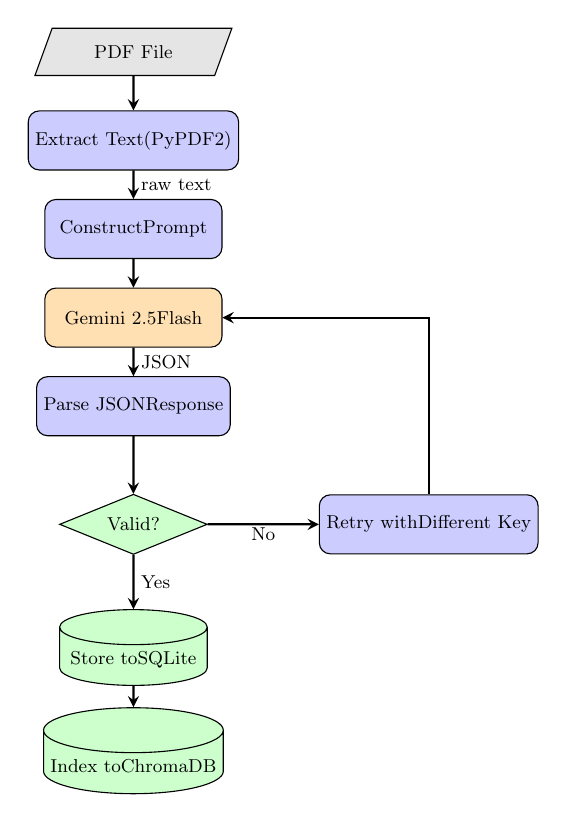
\begin{tikzpicture}[node distance=1.5cm, scale=0.75, every node/.style={scale=0.75}]

% Main flow
\node (pdf) [data, minimum width=3cm] {PDF File};
\node (extract) [process, below of=pdf, minimum width=3cm] {Extract Text\\(PyPDF2)};
\node (prompt) [process, below of=extract, minimum width=3cm] {Construct\\Prompt};
\node (llm) [process, below of=prompt, minimum width=3cm, fill=accentorange!30] {Gemini 2.5\\Flash};
\node (parse) [process, below of=llm, minimum width=3cm] {Parse JSON\\Response};
\node (validate) [decision, below of=parse, yshift=-0.5cm, minimum width=2.5cm, aspect=2] {Valid?};
\node (store) [database, below of=validate, yshift=-0.8cm, minimum width=2.5cm] {Store to\\SQLite};
\node (index) [database, below of=store, yshift=-0.3cm, minimum width=2.5cm] {Index to\\ChromaDB};

% Retry path - moved further right to avoid overlap
\node (retry) [process, right of=validate, xshift=3.5cm, minimum width=2.8cm] {Retry with\\Different Key};

% Arrows
\draw [arrow] (pdf) -- (extract);
\draw [arrow] (extract) -- node[anchor=west, font=\small] {raw text} (prompt);
\draw [arrow] (prompt) -- (llm);
\draw [arrow] (llm) -- node[anchor=west, font=\small] {JSON} (parse);
\draw [arrow] (parse) -- (validate);
\draw [arrow] (validate) -- node[anchor=west, font=\small] {Yes} (store);
\draw [arrow] (validate) -- node[anchor=north, font=\small, yshift=2pt] {No} (retry);
\draw [arrow] (retry) |- (llm);
\draw [arrow] (store) -- (index);

\end{tikzpicture}
\caption{CV Parsing Workflow - LLM-based extraction pipeline with automatic retry mechanism for handling API failures and invalid responses.}
\label{fig:cv_parsing_flow}
\end{figure}

\subsection{Multi-Dimensional Quality Assessment}

We assess CV quality using three metrics: Quality (presentation), Market Fit (job demand alignment), and Completeness (essential sections). Overall score: $Q_{total} = 0.4Q_{quality} + 0.35Q_{market} + 0.25Q_{complete}$ where $Q_i \in [0, 10]$. The LLM generates strengths, weaknesses, and actionable suggestions.

\subsection{Semantic Job Matching}

Our hybrid approach combines vector similarity (fast retrieval) with LLM ranking (accurate scoring). Figure~\ref{fig:matching_flow} shows the workflow.

\textbf{Algorithm 1: Semantic Job Matching}
\begin{algorithmic}
\STATE \textbf{Input:} CV data $C$, filters $F$, top-k $k$
\STATE \textbf{Output:} Ranked job list with scores
\STATE $E_c \leftarrow$ Embed($C$)
\STATE $J_{candidates} \leftarrow$ ChromaDB.Query($E_c$, $k \times 3$)
\STATE $J_{scored} \leftarrow$ []
\FOR{$j$ in $J_{candidates}$}
    \STATE $score, reason \leftarrow$ GeminiRank($C$, $j$)
    \STATE $J_{scored}$.append($(j, score, reason)$)
\ENDFOR
\RETURN Sort($J_{scored}$)[:k]
\end{algorithmic}

% FIGURE 3: Semantic Matching Workflow
\begin{figure}[htbp]
\centering
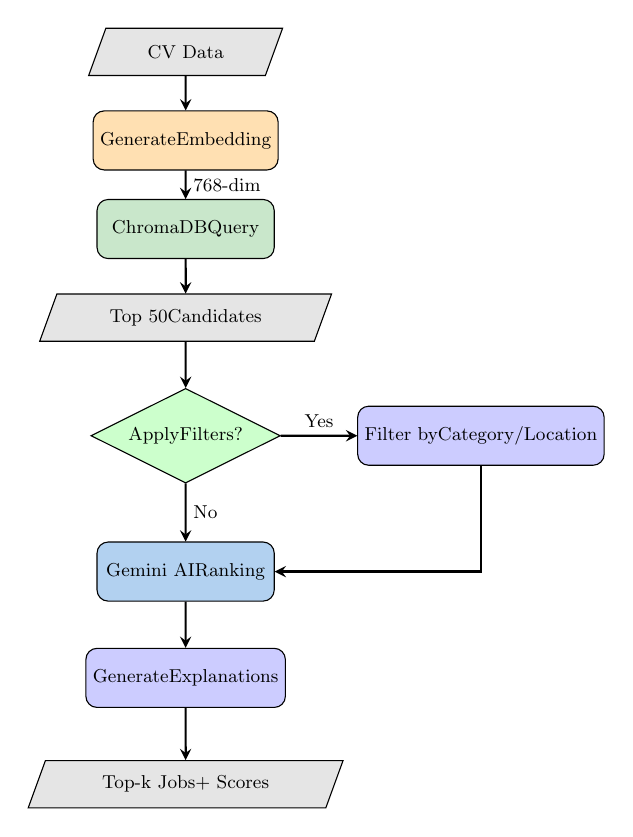
\begin{tikzpicture}[node distance=1.5cm, scale=0.75, every node/.style={scale=0.75}]

% Main flow
\node (cv) [data, minimum width=3cm] {CV Data};
\node (embed) [process, below of=cv, minimum width=3cm, fill=accentorange!30] {Generate\\Embedding};
\node (query) [process, below of=embed, minimum width=3cm, fill=secondarygreen!30] {ChromaDB\\Query};
\node (candidates) [data, below of=query, minimum width=3cm] {Top 50\\Candidates};
\node (filter) [decision, below of=candidates, yshift=-0.5cm, minimum width=2.5cm, aspect=2] {Apply\\Filters?};
\node (rank) [process, below of=filter, yshift=-0.8cm, minimum width=3cm, fill=primaryblue!30] {Gemini AI\\Ranking};
\node (explain) [process, below of=rank, yshift=-0.3cm, minimum width=3cm] {Generate\\Explanations};
\node (results) [data, below of=explain, yshift=-0.3cm, minimum width=3cm] {Top-k Jobs\\+ Scores};

% Filter path
\node (apply_filter) [process, right of=filter, xshift=3.5cm, minimum width=2.8cm] {Filter by\\Category/Location};

% Arrows
\draw [arrow] (cv) -- (embed);
\draw [arrow] (embed) -- node[anchor=west, font=\small] {768-dim} (query);
\draw [arrow] (query) -- (candidates);
\draw [arrow] (candidates) -- (filter);
\draw [arrow] (filter) -- node[anchor=west, font=\small] {No} (rank);
\draw [arrow] (filter) -- node[anchor=south, font=\small] {Yes} (apply_filter);
\draw [arrow] (apply_filter) |- (rank);
\draw [arrow] (rank) -- (explain);
\draw [arrow] (explain) -- (results);

\end{tikzpicture}
\caption{Semantic Matching Workflow - Hybrid approach combining vector similarity search with AI-powered ranking and explanation generation.}
\label{fig:matching_flow}
\end{figure}

\subsection{Retrieval-Augmented Generation for Job Insights}

TalentBridge provides career guidance through RAG, combining vector retrieval with LLM generation. Figure~\ref{fig:rag_workflow} shows the architecture. The indexing pipeline splits each job posting into 3 chunks, embeds them into 768-dimensional vectors, and stores them in ChromaDB with metadata. The query pipeline embeds user questions, retrieves the top-5 relevant chunks, and injects them into Gemini prompts for grounded responses. RAG provides several advantages including accuracy from real data covering 3,237 jobs, insights into current market conditions, specific company and salary citations, and verifiable claims.

% FIGURE 4: RAG Workflow
\begin{figure}[htbp]
\centering
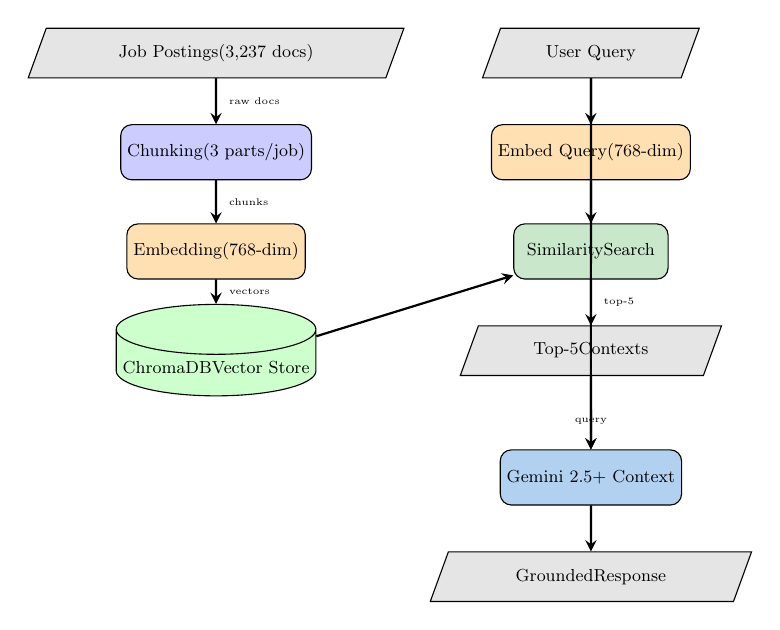
\begin{tikzpicture}[node distance=1.8cm, scale=0.7, every node/.style={scale=0.7}]

% ===== INDEXING PIPELINE (LEFT) =====
\node (docs) [data, minimum width=2.8cm, minimum height=0.9cm] {Job Postings\\(3,237 docs)};
\node (chunk) [process, below of=docs, minimum width=2.8cm] {Chunking\\(3 parts/job)};
\node (embed_doc) [process, below of=chunk, minimum width=2.8cm, fill=accentorange!30] {Embedding\\(768-dim)};
\node (vectordb) [database, below of=embed_doc, yshift=-0.3cm, minimum width=2.8cm] {ChromaDB\\Vector Store};

% ===== QUERY PIPELINE (RIGHT) =====
\node (user_query) [data, right of=docs, xshift=5cm, minimum width=2.8cm, minimum height=0.9cm] {User Query};
\node (embed_query) [process, below of=user_query, minimum width=2.8cm, fill=accentorange!30] {Embed Query\\(768-dim)};
\node (retrieve) [process, below of=embed_query, minimum width=2.8cm, fill=secondarygreen!30] {Similarity\\Search};
\node (top_k) [data, below of=retrieve, minimum width=2.8cm, minimum height=0.9cm] {Top-5\\Contexts};

% ===== GENERATION (BOTTOM) =====
\node (llm) [process, below of=top_k, yshift=-0.5cm, minimum width=2.8cm, fill=primaryblue!30] {Gemini 2.5\\+ Context};
\node (response) [data, below of=llm, minimum width=2.8cm, minimum height=0.9cm] {Grounded\\Response};

% ===== ARROWS =====
% Indexing flow - labels on the right side to avoid overlap
\draw [arrow] (docs) -- node[anchor=west, font=\tiny, xshift=3pt] {raw docs} (chunk);
\draw [arrow] (chunk) -- node[anchor=west, font=\tiny, xshift=3pt] {chunks} (embed_doc);
\draw [arrow] (embed_doc) -- node[anchor=west, font=\tiny, xshift=3pt] {vectors} (vectordb);

% Query flow - no labels to avoid clutter
\draw [arrow] (user_query) -- (embed_query);
\draw [arrow] (embed_query) -- (retrieve);

% Vector DB to Retrieval - label on top to avoid overlap
\draw [arrow] (vectordb) -- node[anchor=south, font=\tiny, yshift=2pt] {} (retrieve);

% Retrieval to Context - label on right side
\draw [arrow] (retrieve) -- node[anchor=west, font=\tiny, xshift=3pt] {top-5} (top_k);

% Context + Query to LLM
\draw [arrow] (top_k) -- (llm);
\draw [arrow] (user_query) -- ++(0,-6.5) -| node[anchor=north, font=\tiny, pos=0.5] {query} (llm);

% LLM to Response
\draw [arrow] (llm) -- (response);

\end{tikzpicture}
\caption{RAG Workflow - Dual-pipeline architecture with offline indexing (left) and online query processing (right) for grounded job market insights.}
\label{fig:rag_workflow}
\end{figure}

\subsection{API Key Rotation}

To overcome Google's free tier quota (50 requests/day), we implement round-robin rotation across three API keys, tripling capacity to 150 requests/day.

\section{Implementation}

\subsection{Technology Stack}

The system is built using Python 3.12, FastAPI, and Uvicorn for the backend. AI capabilities are powered by Google Gemini 2.5 Flash and text-embedding-004 models. Data storage utilizes SQLite 3.x for structured data and ChromaDB for vector embeddings. The frontend is implemented with Vanilla JavaScript, Chart.js for visualizations, and PDF.js for document handling. Additional libraries include LangChain, Pydantic V2, and PyPDF2.

\subsection{Data Collection}

We collected 3,237 real job postings from TopCV, Vietnam's leading job platform. Each posting includes job title and description, company name and industry, location and salary range, experience requirements, required skills, and application deadline. All job descriptions were embedded using text-embedding-004 and stored in ChromaDB for semantic search.

\subsection{Performance Optimization}

Several optimization techniques were implemented to improve system performance. Analytics results are cached for 1 hour to reduce redundant computations. Jobs are embedded in batches of 100 to optimize API usage. FastAPI async endpoints handle I/O operations efficiently. Database connections are pooled and reused to minimize overhead.

\section{Experimental Results}

\subsection{Dataset Statistics}

We collected 3,237 job postings from TopCV. Figure~\ref{fig:dataset_dist} shows distribution: IT (28\%), Business (22\%), Marketing (15\%).

% FIGURE 5: Dataset Distribution Chart
\begin{figure}[htbp]
\centering
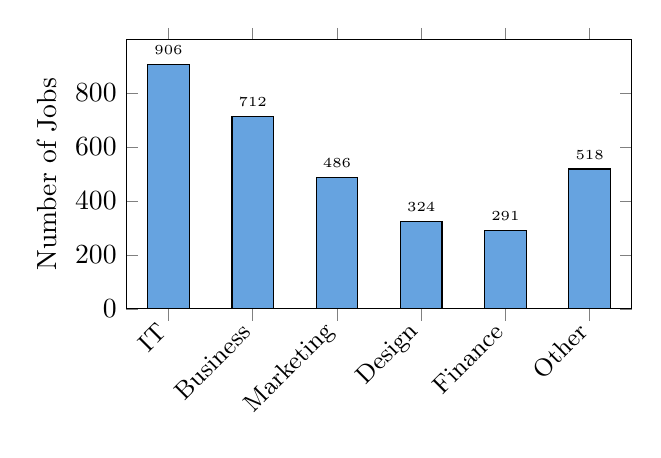
\begin{tikzpicture}
\begin{axis}[
    ybar,
    width=8cm,
    height=5cm,
    ylabel={Number of Jobs},
    symbolic x coords={IT, Business, Marketing, Design, Finance, Other},
    xtick=data,
    x tick label style={rotate=45, anchor=east, font=\small},
    ymin=0,
    bar width=15pt,
    nodes near coords,
    nodes near coords align={vertical},
    every node near coord/.append style={font=\tiny}
]
\addplot[fill=primaryblue!60] coordinates {
    (IT,906)
    (Business,712)
    (Marketing,486)
    (Design,324)
    (Finance,291)
    (Other,518)
};
\end{axis}
\end{tikzpicture}
\caption{Job Dataset Distribution - 3,237 real job postings across 6 major categories from Vietnamese job market.}
\label{fig:dataset_dist}
\end{figure}

\subsection{CV Parsing Accuracy}

We evaluated CV parsing on 50 Vietnamese CVs with diverse formats. Table~\ref{tab1} shows precision and recall for each field.

\begin{table}[htbp]
\caption{CV Parsing Accuracy by Field}
\begin{center}
\begin{tabular}{|l|c|c|}
\hline
\textbf{Field} & \textbf{Precision} & \textbf{Recall} \\
\hline
Personal Info & 98.2\% & 96.5\% \\
Skills & 92.1\% & 88.3\% \\
Education & 95.7\% & 94.2\% \\
Experience & 89.4\% & 85.6\% \\
\hline
\textbf{Average} & \textbf{93.9\%} & \textbf{91.2\%} \\
\hline
\end{tabular}
\label{tab1}
\end{center}
\end{table}

Personal information achieves 98.2\% precision, while experience extraction achieves 89.4\% due to varied formatting.

% FIGURE 6: Parsing Accuracy Chart
\begin{figure}[htbp]
\centering
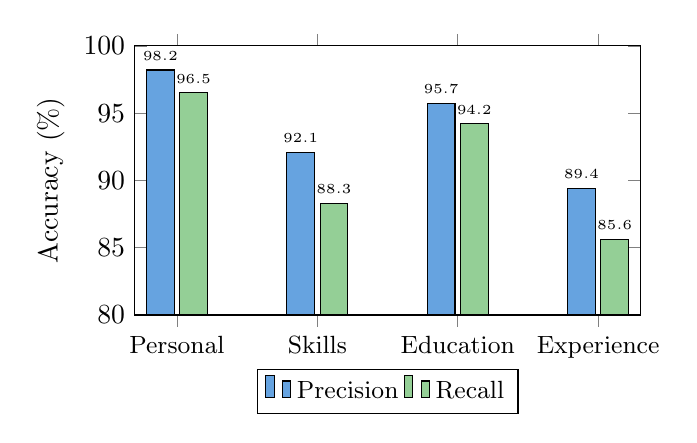
\begin{tikzpicture}
\begin{axis}[
    ybar,
    width=8cm,
    height=5cm,
    ylabel={Accuracy (\%)},
    symbolic x coords={Personal, Skills, Education, Experience},
    xtick=data,
    x tick label style={font=\small},
    ymin=80,
    ymax=100,
    legend style={at={(0.5,-0.2)}, anchor=north, legend columns=2, font=\small},
    bar width=10pt,
    nodes near coords,
    nodes near coords align={vertical},
    every node near coord/.append style={font=\tiny}
]
\addplot[fill=primaryblue!60] coordinates {
    (Personal,98.2)
    (Skills,92.1)
    (Education,95.7)
    (Experience,89.4)
};
\addplot[fill=secondarygreen!60] coordinates {
    (Personal,96.5)
    (Skills,88.3)
    (Education,94.2)
    (Experience,85.6)
};
\legend{Precision, Recall}
\end{axis}
\end{tikzpicture}
\caption{CV Parsing Accuracy - Precision and recall across different CV field categories on 50 test CVs.}
\label{fig:parsing_accuracy}
\end{figure}

\subsection{Job Matching Quality}

30 students rated top-5 recommended jobs on a 1-5 scale. Results: average 4.2/5, 76\% highly relevant (4-5), 8\% not relevant (1-2). 87\% found AI explanations helpful. Figure~\ref{fig:user_ratings} shows rating distribution.

% FIGURE 7: User Rating Distribution
\begin{figure}[htbp]
\centering
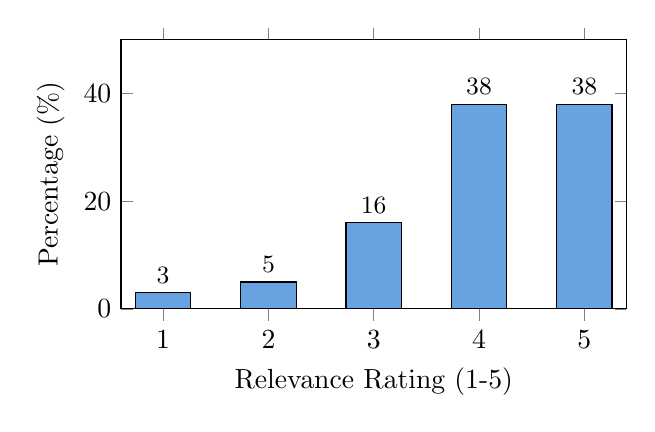
\begin{tikzpicture}
\begin{axis}[
    ybar,
    width=8cm,
    height=5cm,
    ylabel={Percentage (\%)},
    xlabel={Relevance Rating (1-5)},
    symbolic x coords={1,2,3,4,5},
    xtick=data,
    ymin=0,
    ymax=50,
    bar width=20pt,
    nodes near coords,
    nodes near coords align={vertical},
    every node near coord/.append style={font=\small}
]
\addplot[fill=primaryblue!60] coordinates {
    (1,3)
    (2,5)
    (3,16)
    (4,38)
    (5,38)
};
\end{axis}
\end{tikzpicture}
\caption{User Rating Distribution - 76\% of recommended jobs rated as highly relevant (4-5 stars) by 30 student participants.}
\label{fig:user_ratings}
\end{figure}

\subsection{System Performance}

Table~\ref{tab2} shows response times on a standard server (4 cores, 8GB RAM). LLM operations dominate latency (4-7s), while database queries complete in <100ms. Caching reduces analytics time by 98\%.

\begin{table}[htbp]
\caption{System Performance Metrics}
\begin{center}
\begin{tabular}{|l|c|}
\hline
\textbf{Operation} & \textbf{Avg Time} \\
\hline
CV Parse & 4.2s \\
Quality Assessment & 5.1s \\
Semantic Matching & 7.3s \\
Job Search & 0.08s \\
Analytics (cached) & 0.05s \\
\hline
\end{tabular}
\label{tab2}
\end{center}
\end{table}



\subsection{User Interface}

Figures~\ref{fig:ui_landing}-\ref{fig:ui_matching} show the web interface: landing page, CV analysis with quality scores, analytics dashboard, and job matching results.

% FIGURE 9: Landing Page Screenshot
\begin{figure}[htbp]
\centering

\includegraphics[width=0.48\textwidth]{fig/landing_page.png}
\caption{Landing Page - Job search interface with category filters, location selection, and featured job listings.}
\label{fig:ui_landing}
\end{figure}

% FIGURE 10: CV Analysis Screenshot
\begin{figure}[htbp]
\centering

\includegraphics[width=0.48\textwidth]{fig/cv_analysis.png}
\caption{CV Analysis Interface - Upload interface showing parsed CV data, quality scores (Quality: 8.5/10, Market Fit: 7.8/10, Completeness: 9.2/10), and AI-generated feedback with strengths, weaknesses, and improvement suggestions.}
\label{fig:ui_cv_analysis}
\end{figure}

% FIGURE 11: Dashboard Screenshot
\begin{figure}[htbp]
\centering

\includegraphics[width=0.48\textwidth]{fig/dashboard.png}
\caption{Analytics Dashboard - Market insights including job distribution by category, salary ranges, top hiring companies, skill demand trends, and location-based statistics.}
\label{fig:ui_dashboard}
\end{figure}

% FIGURE 12: Job Matching Screenshot
\begin{figure}[htbp]
\centering

\includegraphics[width=0.48\textwidth]{fig/job_matching.png}
\caption{Job Matching Results - Recommended jobs with AI-generated match scores (0-1 scale) and detailed explanations highlighting skill alignment, experience fit, and career relevance.}
\label{fig:ui_matching}
\end{figure}

\section{Discussion}

\subsection{Advantages}

The system offers several key advantages. Automation eliminates manual CV entry, reducing time from hours to seconds. Semantic understanding captures meaning beyond keywords, for example matching "React" with "frontend frameworks". Explainability is achieved through detailed match explanations that help students identify skill gaps. The cost-effective design uses free-tier APIs, making it accessible for educational institutions.

\subsection{Limitations}

Despite its advantages, the system has several limitations. API quota constraints from free-tier limits of 150 requests per day restrict scalability. Latency is increased by LLM calls which add 3-8 seconds per request. Format sensitivity causes accuracy to drop for creative CV layouts. Cold start problems mean new users receive generic recommendations. Language support is currently limited to Vietnamese only.

\subsection{Future Work}

Several directions for future development have been identified. User authentication and personalization with feedback learning will improve recommendation quality over time. A conversational AI chatbot for career counseling will provide interactive guidance. Email and push notifications for new matching jobs will keep users engaged. Mobile applications for iOS and Android will expand accessibility. A recruiter dashboard will add enterprise features for hiring managers. Multimodal CV understanding with vision-language models will handle diverse document formats more effectively.

\section{Conclusion}

This paper presented TalentBridge, an intelligent job matching platform combining LLMs with semantic vector search. Our hybrid architecture achieves 93.9\% precision in CV parsing and 76\% highly-relevant job recommendations with 4.2/5 user satisfaction.

Key contributions: (1) dual-pipeline architecture integrating LLM-based CV analysis with vector matching, (2) multi-dimensional quality assessment, (3) RAG-based career insights, and (4) comprehensive evaluation with real users.

The system demonstrates that modern AI can enhance job search through automation, semantic understanding, and explainability. Open-source availability (\url{https://github.com/Trinhvhao/TalentBridge}) enables further research and deployment in educational institutions.

\section*{Acknowledgment}

The author thanks Google for providing free access to Gemini AI APIs, TopCV for job market data, and the open-source community for the excellent tools and libraries that made this project possible.

\begin{thebibliography}{00}
\bibitem{b1} M. Kenthapadi, B. Le, and G. Venkataraman, ``Personalized job recommendation system at LinkedIn: Practical challenges and lessons learned,'' in Proc. 11th ACM Conf. Recommender Systems, 2017, pp. 346-347.
\bibitem{b2} T. Brown et al., ``Language models are few-shot learners,'' in Advances in Neural Information Processing Systems, vol. 33, 2020, pp. 1877-1901.
\bibitem{b3} Y. Koren, R. Bell, and C. Volinsky, ``Matrix factorization techniques for recommender systems,'' Computer, vol. 42, no. 8, pp. 30-37, Aug. 2009.
\bibitem{b4} C. Wu et al., ``Graph neural networks in recommender systems: A survey,'' ACM Computing Surveys, vol. 55, no. 5, pp. 1-37, 2022.
\bibitem{b5} S. Singh, A. Kumar, H. Darbari, L. Singh, A. Rastogi, and S. Jain, ``Machine learning-based approach for resume parsing,'' in Proc. Int. Conf. Advanced Computing and Communication Systems, 2020, pp. 449-453.
\bibitem{b6} N. Reimers and I. Gurevych, ``Sentence-BERT: Sentence embeddings using Siamese BERT-networks,'' in Proc. Conf. Empirical Methods in Natural Language Processing, 2019, pp. 3982-3992.
\bibitem{b7} Google AI, ``Gemini API Documentation,'' Google AI for Developers, 2024. [Online]. Available: https://ai.google.dev/
\bibitem{b8} J. Devlin, M. Chang, K. Lee, and K. Toutanova, ``BERT: Pre-training of deep bidirectional transformers for language understanding,'' in Proc. NAACL-HLT, 2019, pp. 4171-4186.
\bibitem{b9} P. Lewis et al., ``Retrieval-augmented generation for knowledge-intensive NLP tasks,'' in Advances in Neural Information Processing Systems, vol. 33, 2020, pp. 9459-9474.
\bibitem{b10} A. Vaswani et al., ``Attention is all you need,'' in Advances in Neural Information Processing Systems, vol. 30, 2017, pp. 5998-6008.
\bibitem{b11} S. Robertson and H. Zaragoza, ``The probabilistic relevance framework: BM25 and beyond,'' Foundations and Trends in Information Retrieval, vol. 3, no. 4, pp. 333-389, 2009.
\bibitem{b12} J. Johnson, M. Douze, and H. Jégou, ``Billion-scale similarity search with GPUs,'' IEEE Transactions on Big Data, vol. 7, no. 3, pp. 535-547, 2021.
\bibitem{b13} Y. Liu et al., ``RoBERTa: A robustly optimized BERT pretraining approach,'' arXiv preprint arXiv:1907.11692, 2019.
\bibitem{b14} Z. Yang et al., ``XLNet: Generalized autoregressive pretraining for language understanding,'' in Advances in Neural Information Processing Systems, vol. 32, 2019, pp. 5753-5763.
\bibitem{b15} T. Mikolov, K. Chen, G. Corrado, and J. Dean, ``Efficient estimation of word representations in vector space,'' arXiv preprint arXiv:1301.3781, 2013.
\end{thebibliography}

\end{document}

